%%==================================================
%% chapter3.tex for BIT Master Thesis
%% version: 0.1
%% last update: Nov 8th, 2017
%%==================================================
\chapter{二维参数的信息浓缩估计算法}\label{chap:3}
上面一章介绍了半参数系统中的信息浓缩估计方法,从相关的定理\ref{thm:ic1}可知不同的先验知识会导致信息集合$I_{k}$的形式不同。而从其实施框架可知,一维情形由于只有一个参数不涉及顶点集的组合,因而具体算法比较容易实现,上面第\ref{subsubsect:2.3.3.1}已经给出具体计算步骤。但是实际情况往往不只有一个参数,因而需要设计多维情形的估计算法。多维情形的算法如果直接通过代数推导,不容易解决,需要借助计算几何的思想。在线性控制理论和单变量系统中,两个参数的情况十分常见。因此本章针对两个参数即$d_{1}=2$的情形,设计信息浓缩估计器的具体算法。
\section{问题描述}\label{sect:3.1}
在第二章的基础上,本章继续考虑上下界这种典型的先验知识。如前所述,需要针对关联这种先验知识的系统设计信息浓缩估计算法,完整的过程主要以下分为两步:
\begin{enumerate}
\item 信息浓缩。在上一个时刻的基础上,根据这个时刻的输入输出数据得到的约束,确定这个时刻的信息浓缩之后的参数集合。
\item 选定合适值。根据一定的法则,从上述的参数集合中选择合适的估计值作为这个时刻的参数估计值参与控制律等后续的计算。
\end{enumerate}

第一步的具体操作是,在某个确定时刻得到的一组输入输出数据可以确定两个线性约束不等式,将这个两个约束先后加入到之前时刻的顶点集合中,得到这一时刻的顶点集合,也就确定了当前时刻的参数集合。从理论上说,第一步得到的参数集合中的每一个值都可以作为这个时刻的估计值,但是控制律等后续计算往往需要一个具体的值,所以需要按照一定的法则从集合中确定一个最优值,一般选择多边形的中心作为这个时刻的估计值。上面的两步中,第一步信息浓缩是难点。因此,本章的重点在于第一步的算法设计。一个时刻的信息浓缩过程包含两组约束关系的先后加入,也就是两次$G$变换。这两次的变换过程一样,只是每次的数据不一样,故这里只需要考虑一次变换。另外,为了叙述方便,本章关于时刻$k$的下标省略。

$d_{1}=2$时,用$\beta$和$\beta'$分别表示两个不同的多边形,其顶点集合表示(按顺时针排列,下同)为
\begin{equation*}%
\begin{split}%
\beta&=\{P_{1},P_{2},\ldots,P_{N}\\
\beta'&=\{P_{1}',P_{2}',\ldots,P_{N'}'\}
\end{split}
\end{equation*}

$d_{1}=2$时,关于未知参数$\bm{\theta}$的约束不等式为
\begin{equation}\label{eq.3.L}
\bm{\phi}^{T}\cdot\bm{\theta}\leq e
\end{equation}
这里$\bm{\phi}$和$\bm{\theta}$都是二维向量,$\bm{\phi}$和$e$都可以由输入输出组合得到,$\bm{\theta}$是这个不等式的未知变量。

因此,映射关系$G(\beta,\bm{\phi},e)$可以记为
\begin{equation}%
\mathbf{AddLinear2D}\colon \beta\rightarrow\beta'
\end{equation}
这就是二维参数的信息浓缩估计算法需要解决的核心部分。

\section{几何关系分析}\label{sect:3.2}
记两元组$L=(\phi,e)$表示一条直线。二维情形下主要是考虑同一个平面内,直线和多边形的位置关系。图\ref{fig.2d.export}展示了直线和多边形位置关系的一种可能的例子,从这个图中可以知道求解这个顶点集涉及到计算几何的知识,需要全面考虑各种情形。具体来看,分析一条直线和多边形位置关系,就是考察多边形中每个顶点和直线的位置关系。

记
$$\bm{\phi}^{T}=[\phi_{1},\phi_{2}]$$,
顶点$P_{n}$的坐标为
\begin{equation*}
P_{n}\colon (X_{P_{n}},Y_{P_{n}})
\end{equation*}
则顶点$P_{n}$和直线$L$的位置关系可以由下面的不等式确定
\begin{equation}\label{eq.3.L.P}
\bm{\phi}^{T}\leq e
\end{equation}

\begin{figure}
	\centering
	\subfigure[情形1.1]{	 % Caption of subfigure in []
	\label{fig.poly.1.1}	 % Label of subfigure in {}
	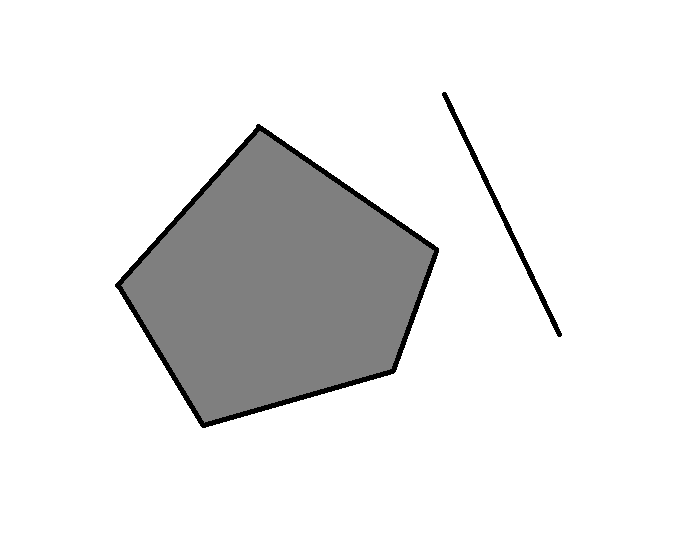
\includegraphics[width=0.45\textwidth ]{ch2-poly-00.png}}
	\subfigure[情形1.2]{
	\label{fig.poly.1.2}
	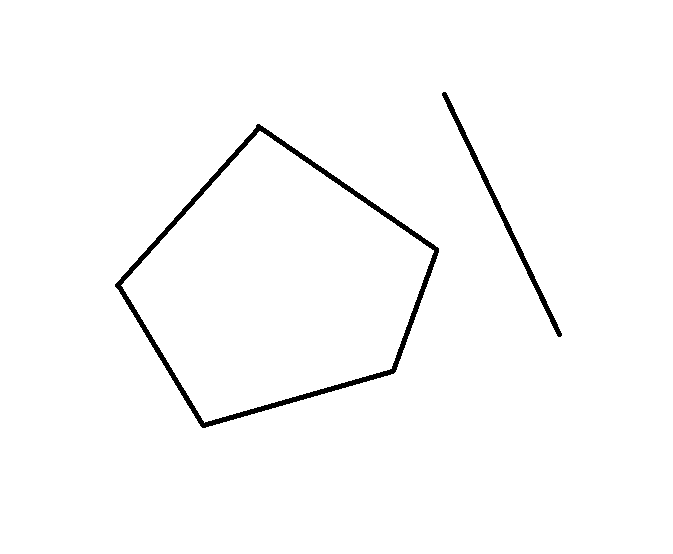
\includegraphics[width=0.45\textwidth ]{ch2-poly-01.png}}
	\subfigure[情形2.1]{	 % Caption of subfigure in []
	\label{fig.poly.2.1}	 % Label of subfigure in {}
	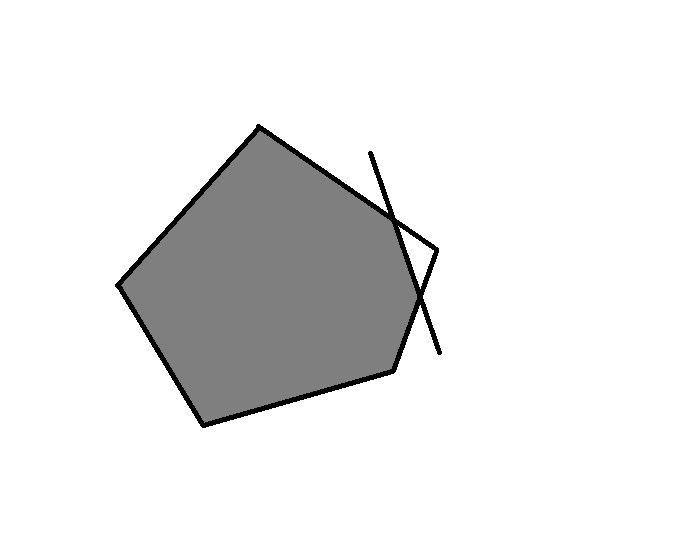
\includegraphics[width=0.45\textwidth ]{ch2-poly-10.png}}
	\subfigure[情形2.2]{
	\label{fig.poly.2.2}
	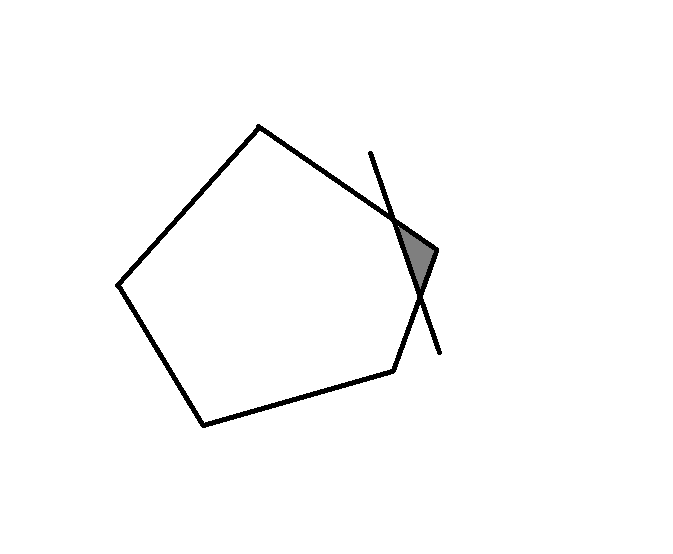
\includegraphics[width=0.45\textwidth ]{ch2-poly-11.png}}
	\subfigure[情形3.1]{	 % Caption of subfigure in []
	\label{fig.poly.3.1}	 % Label of subfigure in {}
	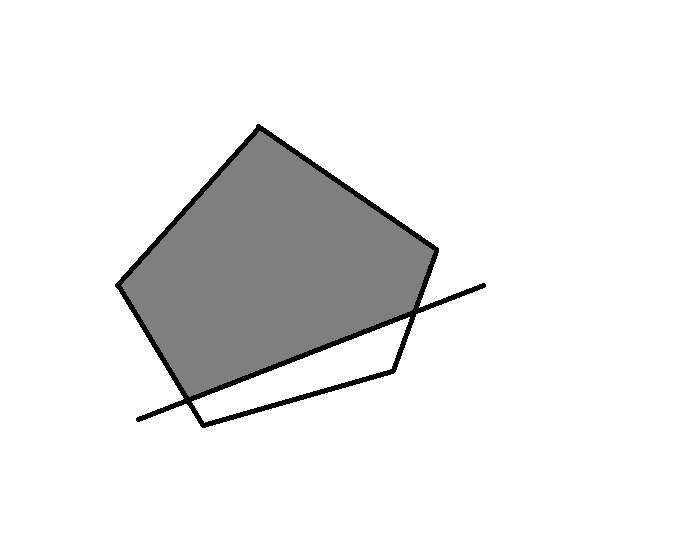
\includegraphics[width=0.45\textwidth ]{ch2-poly-20.png}}
	\subfigure[情形3.2]{
	\label{fig.poly.3.2}
	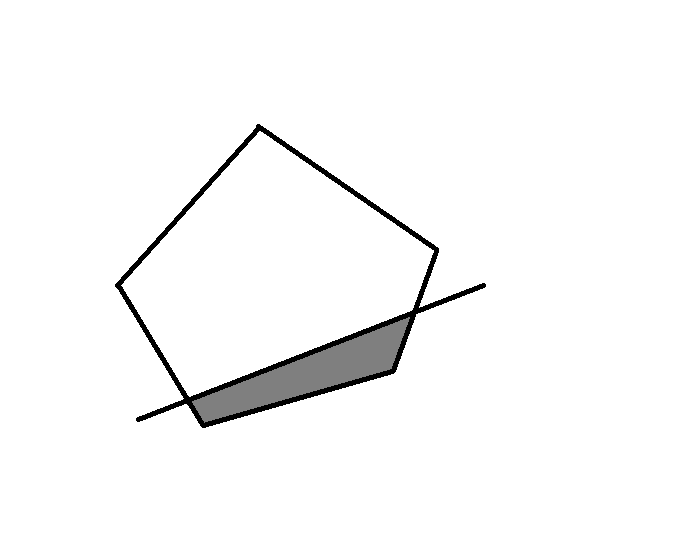
\includegraphics[width=0.45\textwidth ]{ch2-poly-21.png}}
	\caption{直线和多边形位置关系}	 % Caption of figure
	\label{fig.poly.l}	 % Label of figure
\end{figure}

如图\ref{fig.poly.l}所示。

\section{算法实现}\label{sect:3.3}
本章设计了$d_{1}=2$时多边形顶点变换$G$的计算几何算法,具体过程见算法\ref{alg.ic.2d}。

\begin{algo}%
\caption{$d_{1}=2$时多边形顶点变换$G$}
\label{alg.ic.2d}
\begin{algorithmic}
\REQUIRE\\
$\beta$: 顶点集$\{P_{1},P_{2},\ldots,P_{N}\}$\\
\ENSURE
$\beta'$:顶点集$\{P_{1}',P_{2}',\ldots,P_{N'}'\}$\\
\STATE Denote the number of vertices in $\beta$ by $N$
\FOR{$j=1$ to $N$}
	\STATE Denote the $jth$ vertex by $P_{j}$
	\STATE Let $F_{j}=\mathbf{sgn}(c-\phi^{T}P_{j})$
\ENDFOR
\IF{$F_{j}\geq0\ \forall 1\leq j\leq n$}
	\STATE $\beta'\leftarrow\beta$ and return
\ELSIF{$F_{j}<0\ \forall 1\leq j\leq n$}
	\STATE $\beta\leftarrow\emptyset$ and return
\ENDIF
\FOR{$j=2$ to $N-1$}
    \IF{($P_{j}$ and $P_{j-1}$ are in different sides) $\bigwedge$ ($P_{j}$ and $P_{j+1}$ are in different sides)}
		\STATE $P_{1}^{i}\leftarrow$ the intersection of $l_{i}$ and $\overline{P_{j-1}P_{j}}$
		\STATE $P_{2}^{i}\leftarrow$ the intersection of $l_{i}$ and $\overline{P_{j+1}P_{j}}$.
		\IF {($F_{j}>0$)}
			\STATE$\beta'=\{P_{1}^{i},P_{j},P_{2}^{i}\}$
		\ELSE
			\STATE$\beta'=\{P_{1},\ldots,P_{j-1},P_{1}^{i},P_{2}^{i},P_{j+1},\ldots,P_{n}\}$
		\ENDIF
        \STATE break
    \ELSIF{($P_{j},P_{j-1}$ are in different sides) $\bigwedge$ ($P_{j},P_{j+1},\ldots,P_{j+a-1}$ are on the same side) $\bigwedge$ 
		($P_{j+a-1},P_{j+a}$ are on different sides)}
		\STATE $P_{1}^{i}\leftarrow$ the intersection of $l_{i}$ and $\overline{P_{j-1}P_{j}}$
		\STATE $P_{2}^{i}\leftarrow$ the intersection of $l_{i}$ and $\overline{P_{j+a-1}P_{j+a}}$.
		\IF {($F_{j}>0$)}
			\STATE$\beta'=\{P_{1}^{i},P_{j},\ldots,P_{j+a-1},P_{2}^{i}\}$
		\ELSE
			\STATE$\beta'=\{P_{1},\ldots,P_{j-1},P_{1}^{i},P_{2}^{i},P_{j+a},\ldots,P_{n}\}$
		\ENDIF
        \STATE break
	\ELSIF{($P_{j},P_{j+1}$ are in different sides) $\bigwedge$ ($P_{j},P_{j-1},\ldots,P_{j-b+1}$ are on the same side) $\bigwedge$ 
	($P_{j-b+1},P_{j-b}$ are on different sides)}
		\STATE $P_{1}^{i}\leftarrow$ the intersection of $l_{i}$ and $\overline{P_{j-b+1}P_{j-b}}$
		\STATE $P_{2}^{i}\leftarrow$ the intersection of $l_{i}$ and $\overline{P_{j+1}P_{j}}$.
		\IF {($F_{j}>0$)}
			\STATE$\beta'=\{P_{1}^{i},P_{j-b+1},\ldots,P_{j},P_{2}^{i}\}$
		\ELSE
			\STATE$\beta'=\{P_{1},\ldots,P_{j-b},P_{1}^{i},P_{2}^{i},P_{j+1},\ldots,P_{n}\}$
		\ENDIF
        \STATE break
    \ENDIF
	\STATE $j\leftarrow j+1$
\ENDFOR
\STATE return $\beta'$
\end{algorithmic}
\end{algo}
\section{仿真实例}\label{sect:3.4}
仿真曲线如图\ref{fig.2d.theta}所示。
\begin{figure}
	\centering
	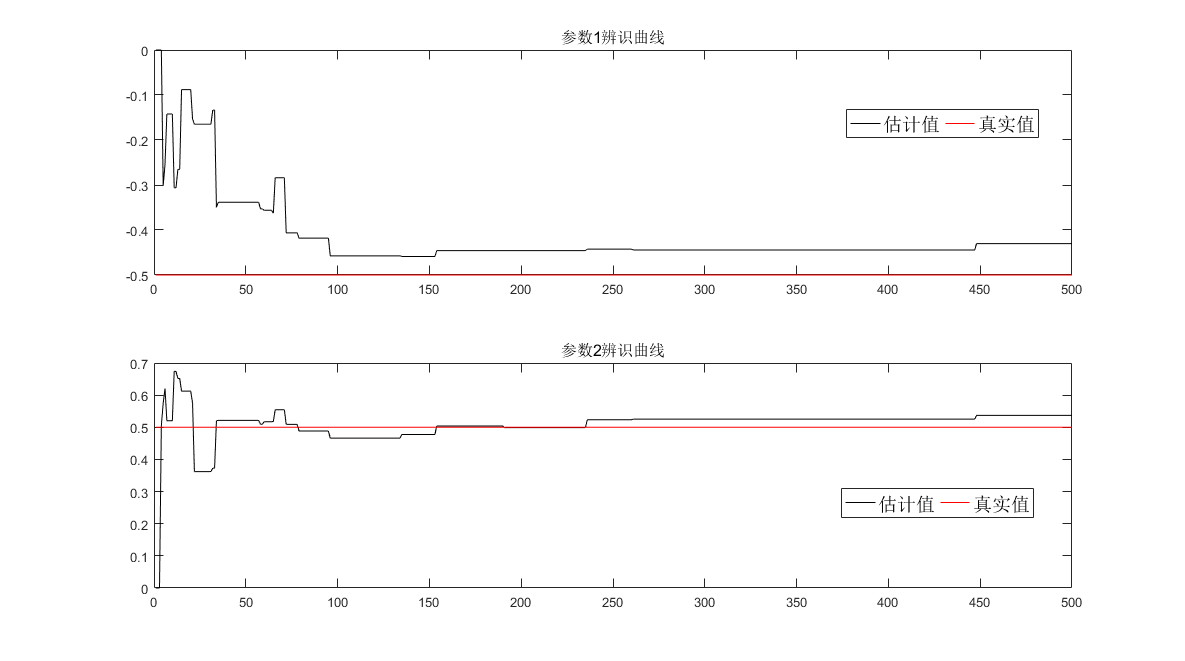
\includegraphics[width=0.7\textwidth ]{ch-2d-theta.png}\\	 % e.g.,[scale=0.75], [width=0.75\textwidth ]
	\caption{$d_{1}=2$时信息浓缩估计参数估计结果}
	\label{fig.2d.theta}
\end{figure}

\section{信息浓缩估计的主要特点}\label{sect:3.5}
半参数自适应控制给出了一种新的理论框架,解决两种不确定性同时出现的系统。现有的半参数自适应控制实现了一维情形下的参数估计算法,但二阶及其以上的参数估计并未具体实现,这涉及计算几何的知识。因此设计高阶情形下基于信息浓缩思想的参数估计算法是实现半参数自适应控制的前提。
